\documentclass[tikz,border=4pt]{standalone}
\usetikzlibrary{positioning}

\tikzset{
  set/.style      = {circle, draw, thick, minimum size=40mm, fill opacity=0.3},
  set name/.style = {font=\bfseries},
  count/.style    = {font=\small},
}

\begin{document}
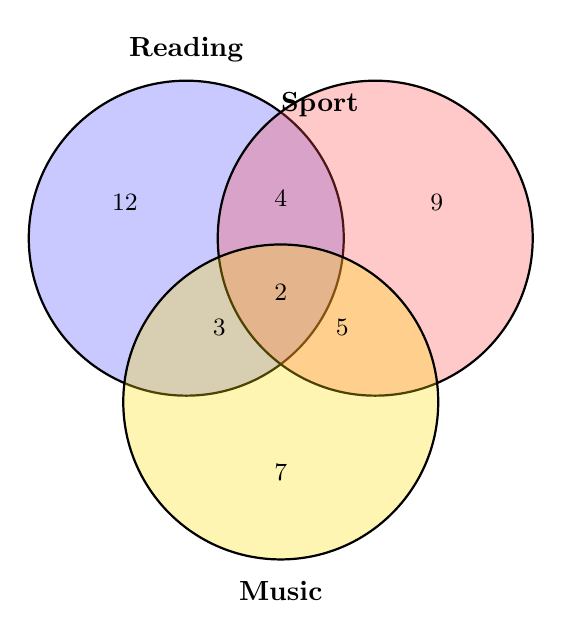
\begin{tikzpicture}[on grid]
  % Three overlapping sets, their centers 24mm apart. The overlaps show
  % through because each circle is filled at 30% opacity.
  \node[set, fill=blue!70]                         (a) {};
  \node[set, fill=red!70]         (b) at (2.4,0) {};
  \node[set, fill=yellow!80!orange, below right=20.8mm and 12mm of a] (c) {};

  \node[set name, above=24mm of a] (reading) {Reading};
  \node[set name, above right=2.4cm of a] (sport)   {Sport};
  \node[set name, below=24mm of c] (music)   {Music};

  % How many belong to each region.
  \node[count, above left=4.5mm and 7.8mm of a]   (only-a)  {12};
  \node[count, right=3.18cm of a, yshift=4.5mm]  (only-b)  {9};
  \node[count, below=9mm of c]                    (only-c)  {7};
  \node[count, above right=5mm and 12mm of a]     (ab)      {4};
  \node[count, below right=11.4mm and 4.2mm of a] (ac)      {3};
  \node[count, below right=1.14cm and 1.98cm of a]  (bc)      {5};
  \node[count, below right=6.9mm and 12mm of a]   (abc)     {2};
\end{tikzpicture}
\end{document}
